\title{Big Data Analytics and Applications in the Travel Industry and Its Potential in Improving Travel Accessibility}

\author{Weixuan Wang}
\affiliation{%
  \institution{Indiana University Bloomington}
  \city{Bloomington} 
  \state{Indiana} 
  \postcode{47405}
}
\email{wangweix@indiana.edu}
 

% The default list of authors is too long for headers}
\renewcommand{\shortauthors}{Weixuan Wang}


\begin{abstract}
Big data applications and analytics have been influencing and improving 
tourists' experience. Travel accessibility refers to provide access for 
people with disabilities or limited mobility (such as seniors), who represent
a growing market in the travel industry by spending billions on leisure and 
business trips. This report explored the implementation of bid data analytics
and applications in tourism, disabilities related studies and assistive technologies
for people with disabilities. This report explored the potentials of big data applications
and analytics in understanding the needs and travel experience of people with disabilities
and improving travel accessibility and quality of life for people with disabilities.
\end{abstract}

\keywords{i523, HID234, Big Data Analytics, Travel Accessibility, People with Disabilities, Quality of Life}


\maketitle



\section{Introduction}
People with disabilities represented a large neglected tourism market. According to
Amadeus annual report, 15 percent of worldwide population (around 1 billion people) lives
with some forms of disability \cite{Ama}. According to United Nation, people with 
disabilities are the largest minority group in the world
\cite{Appleyard2005,DARCY2010816,Lex}. Notably, the number of people with disabilities is
expected to increase as a  result of extension of human life-span, decreases in
communicable diseases, the improvement of medical technology, and decrease of child
mortality \cite{SMITH1987376}.  While some forms of disabilities might be genetic, but
temporary or permanent disabilities can happen to anyone, such 
as spinal cord injury after car accident, or limited mobility at later stage of life
\cite{Lex}. 

Population aging trend also signifies that disability will be a more common
and urgent issue in the future \cite{Grue}. The World Health Organization estimates that
by 2050, 21.5 per cent of the global population will be aged over 65 \cite{Ama}. As a large
and fast growing minority group worldwide, people with mobility limits and accessibility 
issues faces a large ranges of barrier when traveling, and travel and tourism demand of 
this group is often underestimated or completely ignored \cite{Ama}. According to the
Open Door Organization (ODO) market report in 2015, people with disabilities spend 17.3
billion dollars annually for their own travel \cite{ODO}. Because people with disabilities
usually needs a care giver or family member to accompany them when traveling, the potential
economic impact could double \cite{ODO}. 

\begin{figure}[htb]
  \centering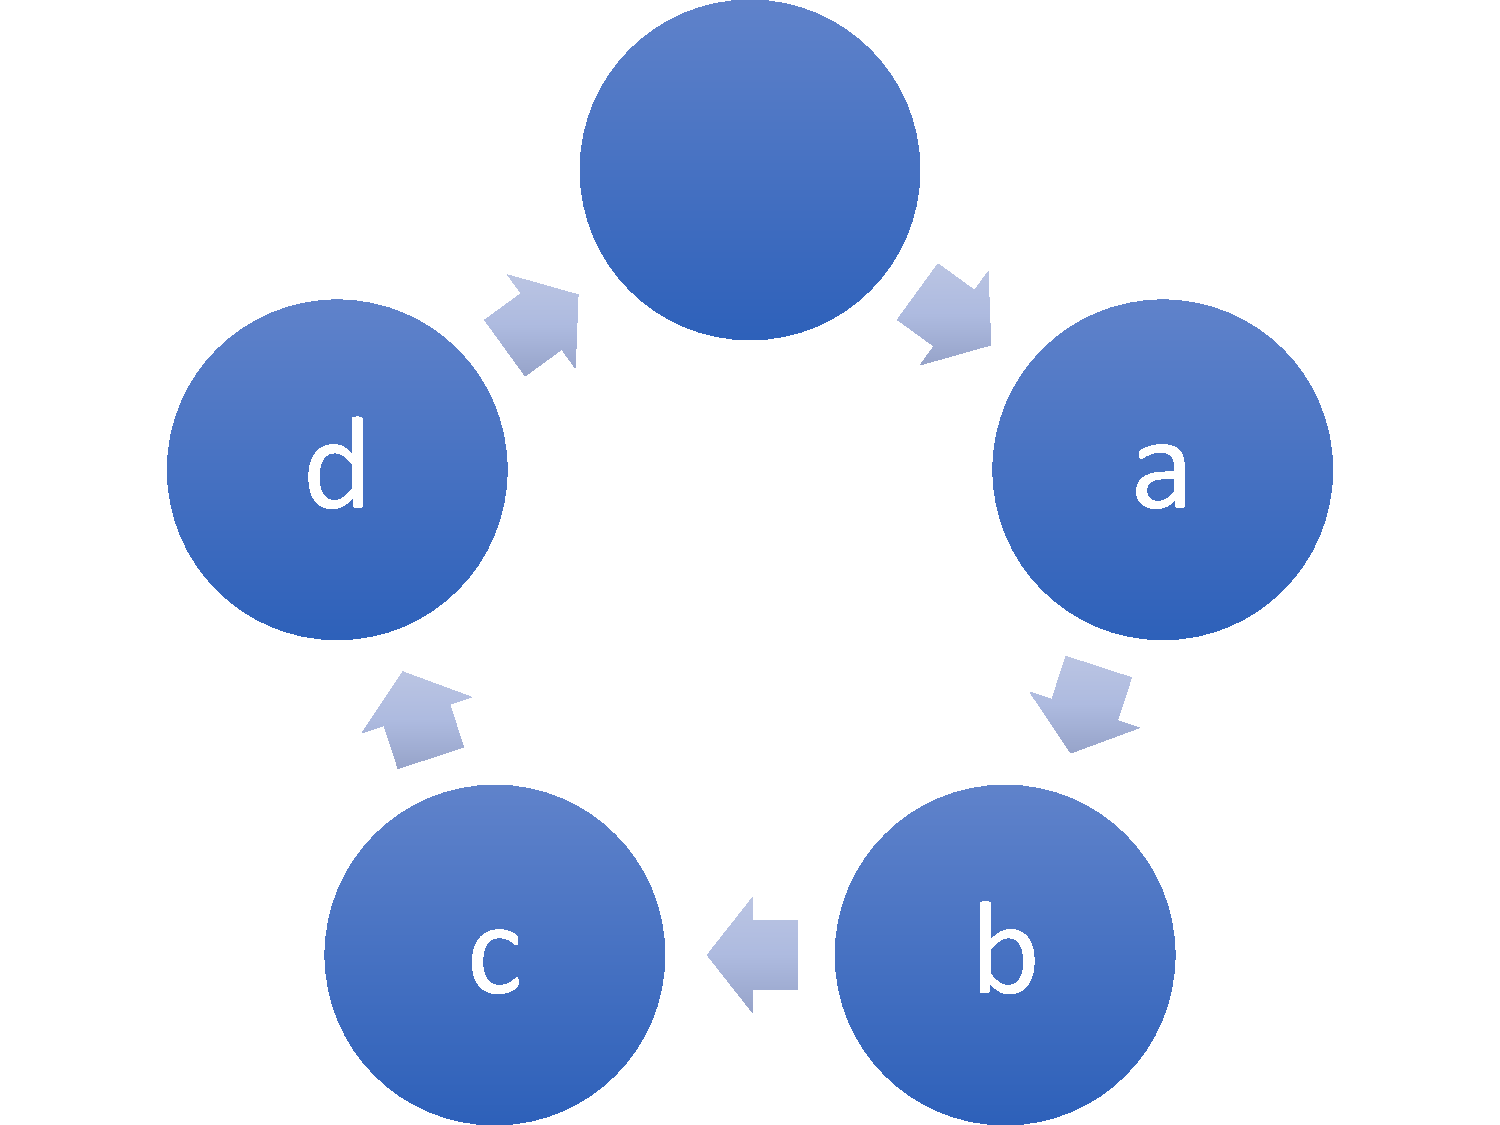
\includegraphics[width=\columnwidth]{images/abc.pdf}
  \caption{put the caption gere \cite{SMITH1987376}.}\label{F:abc}
\end{figure}

\begin{figure}[htb]
  \centering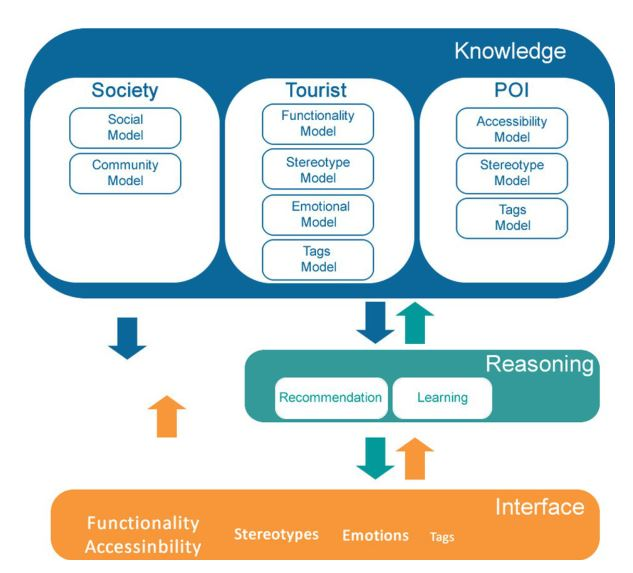
\includegraphics[width=\columnwidth]{images/rec.JPG}
  \caption{put the caption gere \cite{SMITH1987376}.}\label{F:rec}
\end{figure}

As shwon in Figure \ref{F:rec} ....


Accessible travel or accessible tourism refers to the inclusive travel activities that
enable people with access requirements, including mobility, vision, hearing and cognitive
dimensions of access, to function independently, with equity and dignity through the
delivery of universally designed tourism products, services and environments \cite{Ama}.
However, the travel experiences for people with disabilities are more than access
issues. In order to achieve travel accessibility, which means provide travel activities
for people with disabilities, a variety of aspects for travel needs must be taken in
consideration. An accessible destination and appropriate accommodation only lay the 
foundation for a particular travel experience to happen for people with 
disabilities \cite{ODO}. More aspects that need to
consider for people who are traveling with disabilities, such as accessible
transportation, accessible online booking \cite{Ama}.

The ultimate aim for those involved in supporting accessible travel is to empower every
individual to plan and travel independently, at their own will \cite{zhang2016}. However,
the task is not a easy one. Making the whole travel chain accessible, including the
information and booking procedures, as well as the infrastructure and processes become a
important task for travel accessibility \cite{Ama}. 

The development of information communication technologies especially the creation
and distribution of user-generated content (UGC) or consumer-generated content (CGC) has
successfully changed how people travel and how people gather information for travel
\cite{chung2009}. Big data application and analytics has become a trending topic for
the tourism industry and tourism studies \cite{chung2009}. The fast development of 
information and digital technology has changed many people's
lives, especially the life of people with disabilities has also been improved by
technology \cite{GJT14}. People with poor visions can using cell phones to contact
others, access information online with screen readers. People with hearing problems can
text other people with their cell phone. The use of big data for disabilities related
research, disability informatics and developing assistive technology has been studies
to improve the quality of life for people with disabilities \cite{Grue}. 

Although big data is becoming an important topic in both tourism studies and disability
related studies. There are a gap in the literature about how big data can be used in 
accessible tourism practice and studies, the potential of big data analytics and applications
for improving travel accessibility has not been discussed before. Travel for business and
leisure, especially travel independently and with dignity, constitute an essential needs for
people with disabilities, and plays a fundamental part in the quality of life for people with
disabilities. This study is trying to explore the use of big data applications and big data
analytics in tourism and disability
related practice and research, illustrating and discovering the potential of using big data
applications and analytics for accessible travel and tourism practice and studies.

\section{Tourism and Big Data}
Information Communication Technologies (ICTs) have been transforming tourism business
globally and revolutionizing the world of Tourism. It transforms tourism from a
labor-intensive to an information-intensive industry \cite{Williams201787}.
Tourists influence by the developments in search engines, network speed and capacity 
have been using use technologies for better planning and experiencing their
trips \cite{XIE2017101}. In addition, ICTs enable travelers to access reliable and
accurate information and make reservations faster, cheaper and more convenient than
the traditional way \cite{chung2009}. The development of ICTs also enables Internet 
users to both create and distribute information (especially multimedia information), which is called user-generated 
content (UGC) or consumer-generated content (CGC) \cite{chung2009}.

Big data is a new and trending topic in the tourism industry and tourism studies, however, 
it is not unfamiliar to tourist activities. Most activities in the tourism industry had 
been generating a huge amount of data for several years. Booking flight tickets, 
reserving a hotel room and renting a car all leaves a data trail \cite{Shafiee16}.
These data could add up to more than hundred of terabytes or petabytes structured 
data in the conventional databases \cite{akerkar2012}. Discussions of travel planning
on online travel community such as the Lonely Planet Community, status updates and posts 
on social media like Facebook and Twitter, compliments and compliant on review websites 
like TripAdvisor and Yelp, recording and sharing travel experience on travel blogs
constructs more challenging and live unstructured data that arrives at a much
faster pace than a conventional database \cite{akerkar2012}. Tourism practitioners and
tourism scholars are trying to understand tourists' behavior by accepting and analyzing
these big data \cite{Shafiee16}.

Tourists in the digital age often use a variety of tools to access information that
the tourism industry or other users have provided \cite{XIANG2015120}. A tourist
produces a high volume of data when they are searching for travel websites, reporting
issues on mobile applications, sharing traffic information in the cities, searching and
posting on social media, taking and sharing photos, reporting experience on travel
websites and social media, documenting their trips on blogs \cite{akerkar2012, Shafiee16}. 
All these data that are produced constantly can demonstrate tourists' motivation, 
interests, and their planning patterns and so on \cite{XIE2017101}.

Previous studies have demonstrated several different usage and formats of big data in
the travel and tourism industry \cite{XIE2017101}. Social media is one of them that
has a huge effect on the tourism industry. Social media includes social networks,
review sites, blogs, media sharing, and wikis \cite{XIANG2015120}. The exceptional
growth of these data sources has inspired companies and institutions to come up with 
new strategies to understand the socio-economic phenomenon in various
fields \cite{Shafiee16}. Discussions and information sharing on social media are
considered as electronic word-of-mouth (eWOM) that has in some degree substituted
tradition face-to-face word-of-mouth (WOM) for information exchange of tourist
experience \cite{chung2009}. 

Most tourism research utilizing big data are focusing on CGC or UGC, especially
online reviews for a hotel. A recent study conducted by Guo, Barnes and Jia used data
mining approach and linguistic analysis to extract meaning from 266,544 online reviews
for 25,670 hotels \cite{GUO2017467}. They mined their customer review data from TripAdvisor
using a web crawler \cite{GUO2017467}. Through their linguistic analysis of their data 
and cross-comparing with perceptual mapping of the hotels, they found 19 controllable
dimensions that are important for hotels to manage their interactions with visitors
(such as the price for value, check in and check out) \cite{GUO2017467}.

Photo post on photographic sharing website also can also provide extensive information
on the tourists. Previous studies have connected photos posted on Panoramio, Flickr,
and Instagram \cite{GJT14, MIAH2017}. Because when a tourist post pictures on these
websites, their photo is tagged with geographic locations and ordered chronologically.
Therefore analyzing photos posted by tourists can provide a photo density map to
better understand tourists' behaviors, and potentially provide opportunities to detect
atypical tourists behavior and characterize communities behaviors \cite{MIAH2017}. However, the study
also has its own limitation because of the limitation of technology to better exploit
the data \cite{GJT14}. Another study focused on the sequence of locations in shared
geotagged photos by tourist to identify and recommend travel routes which helped the
travel recommender system to generate personalized recommendation according to
interests and time available \cite{MIAH2017}. 

Overall for tourism industry and tourism research, big data has becoming more and more popular. 
Both tourism practitioners and tourism researcher has recognized the
influence of big data and big data sources for tourism development. Big data in the
tourism industry are generated by tourists directly, compared to traditional data sets
that are gathered from surveys, they have argued that these direct data from tourists themselves 
can better represent their true travel experience \cite{GUO2017467}. 
Therefore, big data presented us opportunities to
better understand tourist behavior, their motivations, and interests. 

\section{Disability and Big Data}
There are many different definition of disabilities from different organizations. The most cited official
definition is the 1976 definition of the World Health Organization \cite{Appleyard2005}: ``An impairment is
any loss or abnormality of psychological, physiological or anatomical structure or function; a disability
is any restriction or lack (resulting from an impairment) of ability to perform an activity in the manner
or within the range considered normal for a human being; a handicap is a disadvantage for a given
individual, resulting from an impairment or a disability, that prevents the fulfillment of a role that is
considered normal (depending on age, gender and social and cultural factors) for that individual''. While
people with disabilities are those people who have limitations in their actions or activities resulting
from physical, sensory or cognitive impairments, however, there are many types and levels of disabilities and their
actions and activities are affected differently by their disabilities \cite{Appleyard2005}. The complexity
of disabilities presents difficulties and challenges to accommodate the different needs of people with
disabilities and improve their qualities of life \cite{Datapop}. 

The number of individuals living with some sensory or cognitive impairment or assisting an affected person
is enormous \cite{Riga13}. Researchers has been using disability informatics to better understand people with
disabilities. Disability informatics is a sub-specialty of health informatics that is defined as 
``any application that collects, manages, and distributes information that are related to people 
with disabilities, as well as to caregivers (including familiar members and health care providers) 
and rehabilitation professionals'' \cite{Appleyard2005}. Disability informatics is closely
related to other health informatics areas such as medical informatics, public health informatics
and consumer health informatics, because people with disabilities usually have some secondary
medical condition such as poor health status and increased personal health care needs. 

Gather medical and health information can help to better understand and
accommodate people with disabilities \cite{Riga13}. A study from the early 2000 has identified the
potential of public health informatics for prevention at all vulnerable points in the causal chains leading
to disability and proposed that  applications should not be restricted to particular social, behavioral,
or environmental contexts, but in a more global context \cite{Yasnoff}.  

Another previous research has
designed and deployed an extended version of Artemis system (a cloud system designed to acquire data and
store physiological data of clinical information for real-time analytics) in a hospital. They have
identified that high speed physiological data produced at intensive care units as big data, and the proper
use of such data can promote health, reduce mortality and disability rates of critical condition patients
and create new cloud-based health analytics \cite{Khazaei14}. Research also has shown that many
disabilities are genetic, therefore, bioinformatics has implications in the education of genetic screening
and gen therapy treatments in the future \cite{Appleyard2005}.

People with disabilities usually need some 
assistive technology in their daily life. These technology that assist them to perform basic physical and 
social functions. The use information technology and assistive applications in disability informatics are 
categorized into three areas: virtual, personal, physical. 
\begin{itemize}
  \item Virtual environment refers to use of digital 
technologies like website and the Internet \cite{Appleyard2005}. The digital revolution had and will 
continue to have a profound positive impact on the life of people with
disability by empowering them with the help of digital technologies \cite{Appleyard2005}. However, there are
still access issues in the digital world. One of the barrier is the use of the World Wide Web (WWW or Web).
Therefore, virtual environment for people with disabilities is usually discussed regarding to web 
accessibility. 
  \item Personal Environment refer to having a safe personal environment for people with disabilities. Safety 
monitoring and health monitor devices are essential in this personal environment, which enables a 
safer personal environment and also provide health information for their medical care providers
 \cite{Appleyard2005}. However the ethic of such health monitor devices are always in debate, some believe
 it can be an invasion of privacy and a restriction of personal freedom, others hold the ground that its
 main purpose is to help people with disease or disabilities, since it can alert their caregiver if the
 individual are exposed to harm (such as a person with mental disability and has a history of self-harming,
 these device can prevent unwanted behavior) \cite{cunningham2017cloud}. 
  \item Physical environment refers to the actual living space, traveling environment for people with 
  disabilities. People with mobility disabilities, visual impairment or cognitive limitation all need 
  special help in their physical environment. Since the American Disabilities 
Act passed in the 1990s, the accessibility of physical environment has been
improved in a great degree. However, people with disabilities still would meet some barrier and problem, 
one of them is the lack of curb cuts. Assistive information technologies has been developed in an effort to
solve this problem. One of them is MAGUS, which is a project using geographical information system to inform 
users about wheelchair accessibility in urban areas \cite{Appleyard2005}
\end{itemize}





The contribution of Big data and cloud computing have been recognized and accepted by researchers in 
health informatics \cite{7047725}. The potential of big data and cloud computing for disability 
informatics and for people with disabilities has 
been explored by a few researchers and organizations. Data-Pop Alliance is one of the organization has recognized 
the big data and potential for study and help people with disabilities for disability informatics and people 
with disabilities \cite{Datapop}. Their research has categorized three type of big data source used across disability
research: exhaust data (mobile-based data, financial transaction, transportation and online trace), digital 
content (social media and crowed-sourced/online content), and sensing data (physical and remote) \cite{Datapop}. 
They also provided the potential for some of these data sources, for example, researchers can use transaction 
data to compare cost, availability, and use of services that offer accessible options (such as accessible hotel 
listings) \cite{Datapop}. They also suggested that researcher can use social media data to represent people with
disabilities as a network of interaction and using crow-sourcing to map the locations of accessible businesses 
and public places \cite{Datapop}. 
The organization has also identify four functions of big data on disability:descriptive, predictive, diagnostic 
and engagement. Descriptive function of big data is to describing and presenting the collected information such
as using location data to map workplaces that are accessible to people with disabilities \cite{Datapop}. 
Predictive function is making inferences based on collected information such as discovering trends in the 
growth of number of accessible businesses in a certain urban area, while the diagnostic function means
establishing and making recommendations on the basis of causal relations such as showing what can help 
increasing accessible business in a certain area \cite{Datapop}. Finally, the engagement function refer
to shaping dialogue within and between communities and with key stakeholders through communication of data \cite{Datapop}.


Cloud computing in combined with big data can also provide great opportunities for research and improvement of
quality of life for people with disabilities \cite{Caldwell2011}. The term cloud ``refers to everything a user may reach via the 
Internet, including services, storage, applications, and people'' \cite{Hoehl2010}. Depending on the type of 
using, the ``cloud'' can be use for different purpose, such as for companies, the cloud could be used for hosting
services so as to avoid the costs and difficulties associated with hosting one’s own servers and software and for
individuals, the could is often used as information storage \cite{Khazaei14}. Regardless of the types of usages 
for cloud, the end using must still access the information and services residing in the cloud through device like
a smart phone or computer \cite{Hoehl2010}. Cloud computing has been used to provide more accessible virtual 
environment, especially Web access through project like WebAnywhere, which is a cloud based tool for blind using 
to access Internet \cite{Hoehl2010}. 

Cloud computing and big data analytics can also be helpful in health monitoring. The Artemis project mention earlier
provide a example of big data analytics and cloud computing usage in health monitoring, by creating new cloud-base
health analytics solutions \cite{Khazaei14}. Previous researchers have developed a mobile app to collect motion 
data of Parkinson's disease (PD) which is a disease resulting in mobility disorder using the smart phone 3D 
accelerometer and to send the data to a cloud service for storage, data processing, and PD symptoms severity
estimation, which provide an user-friendly and economically affordable system to monitor and assess the condition
of PD \cite{info:doi/10.2196/mhealth.3956}. Although this system is not for people with disabilities, but it 
provided potentials for similar systems to be developed for different kind of disabilities. 

Another application of cloud computing and big data in assistive technology is the CloudCast platform, which is a 
cloud-based speech recognition services that can be used for many assistive technology application for people
with speech difficulties and hearing impairment, it also facilitate the collection of speech data required for
the machine learning techniques \cite{cunningham2017cloud}. Similar to Alexa Voice Service, it provide reliable 
speech recognition which can be used with assistive devices for people with hearing impairments, but CloudCast
platform also provide customization for assistive technology applications benefiting users with speech 
impairment \cite{cunningham2017cloud}. This research provided a great example of using big data and cloud 
computing in combine to solve a certain problem for people with disabilities (in this case it is barriers for speech impairment). 

The development of information technology and assistive technology has improved the life of people with disabilities.
The use disability informatics and health informatics can help researchers and service and technology providers 
to better understand the needs and wants for people with disabilities. Studies has discussed and proposed the 
great potentials to use big data source to better represent people with disability and identity and study 
issues and propose actions and solution to the challenges faced by people with disabilities. Using Cloud 
computing and big data also helps improving assistive and information technology that are now used to 
help people with disabilities. To improve the quality of life for people with disabilities, travel as a 
necessary needs and right for human cannot be ignored and the travel demands from the population with 
disabilities have to be addressed. Therefore, it will be beneficial and necessary to study travel 
accessibility with the help of big data and digital technologies, in order to improve the quality of life for people with disabilities. 

\section{Travel Accessibility and Big Data}
To explore the potential of big data applications and analytics in improving travel 
accessibility, the complexity of travel accessibility have to be addressed. 
Accessible travel includes not only the point-to-point transportation (such as air
travel, flights), but also the accessibility of destination \cite{Ama,DARCY2010816,milo}.
For people with disability to actually make the trip, they will also require booking for
transportation and hotel reservation to be accessible. This study is going to 
explore the use of big data application and analytics in different aspect of 
travel such as reservation, long distance 
transportation (in the form of airline travel), and destination transportation,
the existing evidence and potentials for using these big data to improve travel 
accessibility.. 

\subsection{Big data and online reservation}
Nowadays, the majority of the travel planning process happens online. Tourists would
use a variety of tourism website, search engines, and reservation domains. The 
Internet also plays an important part at during and post travel stage, as tourists 
report issues on mobile applications, share traffic information in the cities, 
search and post on social media, take and share photos, report experience on 
travel websites and social media \cite{akerkar2012, Shafiee16}. These activities 
seems mundane and easy to complete for the general public, but for people with 
disabilities they can huge hassles or barriers.

Previous studies in relation to disability informatics  demonstrated 
the profound positive impact of  that the digital revolution on the life
of people with disability by empowering them with the help of digital 
technologies \cite{Appleyard2005}. However, there are still access issues 
in the digital world, the most urgent one is the use of the World Wide Web 
(WWW or Web). The Web has always had a strong awareness and been advocacy 
for accessibility since early on in its evolution \cite{Appleyard2005}. 
The World Wide Web Consortium (W3C) had passed the Web Accessibility Initiative
(WAI) and Web Content Accessibility Guidelines in the late 1990s \cite{Appleyard2005}. 

A number of assistive technologies were designed to help people with 
disabilities to use the Web. For example BBC Education Text to Speech 
Internet Enhancer (BESTIE) is a CGI Perl script that can help people 
with disabilities who are using text-to-speech systems for Web browsing 
to modified the web page removing images, Java and Javascript code
that may cause difficulties to understand the BBC web page content \cite{Erra}. 
However, the limitation of BESTIE is that it is only compatible with BBC 
website. Other researchers also came up with Personalizable Accessible 
Navigation (PAN), which is a set of edge services designed to improve 
Web pages accessibility which allow  personalization and the opportunities 
to select multiple profiles, making it compatible for web as well as mobile 
devices \cite{info:doi/10.2196/mhealth.3956}. 

The online sector of the tourism industry has quickly adopted big data 
applications to better understand the need of customer and to improve 
online experience for customers \cite{akerkar2012}. The online sector 
of the industry include  meta-search engines (like Google), online 
travel agencies (like Expedia) and some information website companies 
that distribute tourism information (TripAdvisor)\cite{MIAH2017}. 
Amadeus, a tourism company known for its global distribution system, 
has developed a program ``Amadeus Airline Cloud Availability'' that 
can generated special result and increase search for its customers \cite{Shafiee16}.

Travel domain companies like Marriott, Southwest airline, and Amtrak 
also developed assistive devices specially for people with disabilities 
to use when browsing their websites. These assistive technologies can 
help people with disabilities to navigate online reservation website, 
and help them to independently booking their travel reservations for 
hotels, restaurants, airplane tickets and attraction passes.

These assistive devices was design to help people with disabilities 
to have access to the Web. However,  current web accessibility standards 
do not respect disability as a complex and culturally contingent interaction.
The needs and demand of people with different types of disabilities are 
certainly not the same and this make it hard to understand and pinpoint 
the real needs for people with disabilities to access the Web. Researchers 
have proposed to use big data to better understand of the relation between 
disability and technology and recognized the difference of disabled people 
in the ``Global South'' where different contexts constitute different 
disabilities and different experiences of web access \cite{Appleyard2005}.

\subsection{Accessible transportation and big data}
An inaccessible transport network prevents many people from going to school 
or studying, working, going to the doctor, meeting friends, going shopping 
or to the cinema and other activities that are taken for granted. However,
for people with disabilities, an inaccessible transport
network would left them dependent and confined in their own home \cite{Ama}. 
More importantly an inaccessible transport network would also prevent people with disabilities to
travel for business or leisure \cite{milo}.
Older adults, people with disabilities, individuals in low-income households, especially 
those living in rural areas can face significant mobility challenges \cite{moya2016dynamic}. 

Concerns about getting into an accident, congestion,
price of travel, access to transit, and lack of walkways are important issues for a large
percentage of the population, but they tend to be more important for people with
disabilities \cite{moya2016dynamic}. For today's travel and transportation businesses,
it is important to address the issue of inclusion, which is the potential to enable 
a broader range of  people to use
transportation infrastructure regardless of their individual abilities or disabilities
\cite{milo}. Accessibility transportation is essential for travel accessibility, 
because it represent two aspect of travel accessibility: 
first is long distance transportation accessibility, and the second is accessible destinations. 
For a destination to be accessible, 
it have to have an accessible transport network allow people with disabilities 
to navigate with the destination.


\subsubsection{Airline and big data}
The airline industry is very familiar with big data use in their daily operations
and market research. Airline companies have been using their big data which is 
the large volume of structured information that has been produced internally 
\cite{MIAH2017} to analyze prices of plane ticket. Moreover, airlines 
have optimized the details of planning for the crew and routing \cite{Shafiee16}. 

Previous studies in airline network used Big Data mined from the U.S. air 
transportation system over the years from 1998–2014 to characterize the 
network's behavior and determine what internal and/or external drivers result 
in structural changes to the airline network \cite{7777957}. Airline delay 
patents has also been studied with the help of big data by identifying by the 
number of late arrivals as a percent of total operations \cite{Sor}. 

In another previous study, researchers used data from 2006 to 2008 in order 
to provides the result about the total flight delay for a specific period of 
time caused due to climate, security, carrier, National Aviation System, Arrival
and Departure based on total number of flights getting delayed over in the 
given period of time \cite{Sor}. In the study, the authors used time series 
analysis along with the integration of heterogeneous database to identify and 
achieve the Airline Seasonal Delay which is implemented and visualized in R, 
they were able to identify a trend line to provide the insights for the aviation
industry to take future measures to avoid delays and manage them \cite{Sor}.

Airline studies have also used big data analytics on passenger reviews data.
The advance development of social media and mobile helped the passengers to 
post reviews in a ubiquitous way, allow them post real time feedback over 
Facebook, Twitter on airports, airlines, and other travel providers
\cite{CHEN2016285}. However, passengers' review can be really complex 
since travel activities usually involve multiple parties, therefore, the
travel domain application systems are also typically managed by different 
stakeholders like airlines, airports, travel agencies, security and other 
services providers like cars, bus, trains, hotels, events. In order to 
provide a holistic approach to manage complex passenger reviews with data 
gathering, processing and disseminating, a previous study has proposed a 
reference architecture to manage passenger reviews where multiple 
stakeholders are involved by using data lakes, which can store, manage 
and analyze structured and unstructured data with cheaper cost, 
well-distributed, open sourced and powerful set of tools.

Even though previous studies on airline using big data have not address the issues 
of accessibility. These previous studies still show the potential for using big data 
source from the airline industry and passenger reviews to study the interests, 
motivation, needs and demands from people with disabilities.



\subsubsection{Transport Network accessibility and big data}
Accessibility in the transport network studies are different defined than travel 
accessibility, since the urban accessibility is focus on provide access of 
transportation and transit to general public, not specifically people with 
disabilities \cite{moya2016dynamic}. However, since transport network accessibility 
usually are connected to urban transport network, which represent an important 
part of physical environment for people with disabilities it can provide some insight for 
accessible destinations especially urban destinations. Accessibility has always been a key 
concept in urban and regional planning for its capacity to link the activities 
of people and businesses to the possibilities of reaching them effectively. 
The accessibility of the transport network is already challenging for general 
public, for people with disabilities who requires special needs, it become a 
tremendous and difficult barrier, because they are required to make rapid, 
real-time decisions that are especially difficult for special needs populations. 
Therefore, previous studies using big data on urban accessibility can provide 
some potentials for travel accessibility studies \cite{Barbeau}.

For Urban an regional planning, accessibility represent traffic capacity to link the 
activities of people and business to the possibilities of reaching them effectively 
\cite{moya2016dynamic}. Accessibility is defined as ``a dynamic attribute of locations
that varies over time due to changes in the transport network and in the attractiveness 
of destinations for certain activities'' \cite{moya2016dynamic}. Since the emergence of
big data generated by social media, smart phones, satellite navigation system and other 
technologies,  the information on transport networks has improved conclusively in recent 
years \cite{Barbeau}. Navigation companies such as TomTom; websites and applications 
like Bing Maps, Google Map; collaborative projects like Open-Street-Map; the public 
availability of Transit Feed Specification and data from other transit authorities 
opens up a rapid growing field of research on real time and time-of-day variations 
in private and public transit accessibility \cite{moya2016dynamic}. These companies 
and institutions have increasingly detailed systems with information on the features 
of roads and public transport networks, and their databases include information on 
speed variations on the roads and the frequencies of passage in public transport
networks, all of which contribute a more efficient and dynamic vision to urban 
accessibility studies \cite{moya2016dynamic}.

Researchers have just started  using these new information sources in 
studies on urban accessibility. Previous studies utilized data obtained from 
global positioning system devices to calculate speeds, congestion levels and 
accessibility conditions at  different times of day (morning, midday, evening,),
other studies analyzed data from Be-Mobile system (which provided the geo-located 
positions of 400,000 vehicles equipped with tracking devices) to calculate car 
travel times \cite{moya2016dynamic}. 

Previous studies also have gathered and analyzed information from web services 
(such as Google map API) to calculate travel times between origins and destinations. 
These studies were able to use new information source and big data provided by the 
development of technologies to retrieve information about local locations and traffic 
condition for local facilities like groceries, malls, restaurants, banks, recreation 
centers and others, and estimate accessibility by car, walking, cycling and public 
transit options \cite{moya2016dynamic}. Previous research also used data from social 
media such as Twitter in combined with data from satellite navigation system (like TomTom) 
to provide a dynamic approach and obtain profiles that highlight the daily variations 
in accessibility in urban cities, identify real time influence of congestion and 
population location changes, by providing different accessibility profiles from 
different transport zone, the researchers was able to analyze the relationship between 
the performance of the transport network and the attractiveness of the destination 
\cite{moya2016dynamic}. Although this study is not design to provide information for 
people with disability, but such dynamic approach using real time big data can also 
benefit people with disabilities and help them identify places to go in the city and 
the most accessible route to the attractions. 

Another study also proposed and developed a travel assistance device for people with 
disabilities by using real time data from global positioning system. According to 
this study, recent advancements in mobile technology enabled smart phones with global 
positioning system provide real-time location-based services and its related data.
The researchers for this study designed, implemented and tested a travel assistance device (TAD) 
that is designed to help transit riders with special needs using public transportation
\cite{Barbeau}. This device is a navigation software program designed to prompt 
individuals via a cell phone to exit the bus at a pre-set location. 
This travel assistance device provides the people with disabilities 
customized real-time audio, visual and tactile prompts for exiting the transit vehicle 
by announcing ``Get ready''and ``Pull the cord now!'', based on  its real-time assisted 
GPS data provided by the embedded GPS chip in the cell phone \cite{Barbeau}.  
Once the software is downloaded and installed to the cell phone,
parents, travel trainers, or other authorized individuals can access the web management
page to schedule bus routes to be transmitted to the cell phone \cite{Barbeau}.  The system also 
provides alerts to riders, their caretakers and travel trainers when the rider with 
disabilities deviates from the planned route. With a website allowing easy access 
for the design and planning of new trip itineraries, the device allows authorized 
personnel (usually caregivers, family members) to monitor the rider’s location 
in real-time from any computer \cite{Barbeau}. The travel assistance device was 
catered to the needs of people with disabilities, increasing their level of 
independence and their care-takers security. This travel assistance device 
represented beneficial practice for people with disabilities \cite{Barbeau}.

However, there are still many challenge for the development of such device or services. 
One of the main challenge is that different needs of people with disabilities
making it difficult to complete satisfy and assist people with different disabilities. 
Since the device proposed by this study is still at experimental stage and their 
test sample are limited, although through the test, the device was proved to be 
easy to use, it still might pose as a challenge for other people with disabilities, 
especially people with cognitive limitations \cite{Barbeau}. 


\section{Promises of Big Data in Travel Accessibility}
As mentioned above, big data has some potentials in studies and research that are intended 
to enable and improve the ability for people with disabilities to travel independently. 
This section are going to explore different big data related technologies, applications and 
analytics that can help people with disabilities to travel with ease and researchers to 
better understand the demand and need for people with disabilities.
\subsection{Internet of Things and Travel Assistive Technology}
\subsubsection{Internet of Things Assistive Technology and Potentials for Travel use}
Assistive devices or technology (AT) for people with disabilities are not a new concept. 
Assistive devices refers to ``any item, piece of equipment, or product system, 
whether acquired commercially off the shelf, modified, or customized, that is used 
to increase, maintain or improve functional capabilities of individuals with 
disabilities'', for examples, canes, crutches, walkers, wheelchairs, and shower 
chairs, hearings aids, visual aids, other hardware, and software that improve 
ICT access or communication capacities are all assistive devices \cite{Barbeau, Shah}. 
People with disabilities are usually seen as depend, and in need of help from
caregiver or family members \cite{YE20096527}. However, with the technological growth that has 
been seen in the last 20 years, a wide array of devices have been adapted, 
created, and utilized with the potential to create independence for individuals 
with disabilities. Virtual reality, sensor monitoring devices, smart phone have 
all been used to assist those who require assistance in their day to day 
lives \cite{moya2016dynamic}.  

Older adults and individuals with physical, sensory, and mental/cognitive 
disabilities encounter many barriers to inclusion and accessing various 
opportunities and services that the society has to offer \cite{Shah}. 
In order to overcome these barriers, people with disabilities needs some 
forms of assistive technologies or devices. Traditional technologies has 
many challenges, however,  with the development of technology, the 
Internet of Things (IoT), smart homes, smart buildings,
smart cities, and other smart environments can overcome some of 
these challenges due to their prevalence and diverse capabilities \cite{Farm}.

One of human's fundamental needs is the mobility and capability of 
independently traveling around, including for people with physical 
disabilities and even blind or visually impaired individuals \cite{Barbeau}.
In order for people with visual impairment to independently travel or 
moving around requires indoor and outdoor navigation capabilities, the 
blind and visually impaired people may rely on some type of AT to 
supplement their navigational abilities \cite{Shah}. Previous studies has 
proposed using the advanced sensors of the smart phones in providing 
meaningful interactions with the environment for individuals 
with different abilities \cite{Shah}. A typical modern smart phone 
has more than twenty sensors, which include GPS-based systems that 
can be useful for outdoor navigation, however in general, these 
sensors in smart phone still may lack the required precision 
and reliability for use by the blind or partially sighted individuals \cite{Shah}. 

Previous research has proposed using Bluetooth beacons and audible 
instructions delivered through an interface device for navigation 
by the blind and partially sighted people is based on the use of 
such as bone conduction earphones or smart phones \cite{Barbeau,Shah}. 
A research team has designed and tested a system ``with 16 Bluetooth beacons 
providing pin-point accurate indoor location mapping'' 
for unassisted mobility in the London Underground \cite{Shah}. The system is based on a mobile app, Wayfnder,  which is 
a open platform that has the promise of promoting future 
development on assistive devices for people with visual limitations \cite{Shah}. 
Microsoft, Guide Dogs, UK and several other organizations have also embarked
on expanding similar concepts to respond to the challenges that people with sight
loss face while navigating the cities \cite{Shah}.  These companies and organizations
has developed technology and application that allow users to start a trip and they 
have a ``Look Ahead'' and ``Find the way'' mode that can help people with vision
limitation to explore the city and let them stop at any point and check 
that they are heading the right direction \cite{Barbeau}. 

\subsubsection{The big data challenge of IoT based AT}
While the growth and progress the IoT and smart
environments, technologies such as sensor technologies for comprehensive
monitoring and surveillance progress and advance unbelievable fast, nevertheless,
there still existed many challenges for these  technologies \cite{Shah}. 
One of the most important challenges is data availability. Because these technologies generated an
enormous amount of data that surpasses the processing and use capabilities \cite{Shah}. For
instance, real-time localization and navigation systems that are designed to assist people 
with visual impairment to travel around, face two major related challenges: one is 
the allocation of computational resources that can process the large
amounts of data coming from multiple sensors and cameras, fast enough in a real-time
and synchronized manner, so that they can provide real-time guidance for people 
with special needs \cite{Shah};the second issue relates to quick and real-time access to
dynamic data sets through interfaces that are appropriate for the user \cite{Shah}.IoT devices 
typically have the issues of energy constrained, with small memory, limited processing 
power, and restrictive communication capabilities \cite{Shah}. One positive aspect of this 
challenge is, these dynamic data obtained from IoT based AT device are extremely 
valuable and could help researchers and companies to better understand the 
needs of people with disabilities and analyzing such data can help researchers 
and companies to design better product for people with disabilities \cite{dewsbury03}.

Another issues that AT adoption faces is its ability of meeting the users’
needs and desires \cite{Shah}. AT has been criticized because although AT devices ``…may have
technical merit, and may solve obvious problems, but still fail to address the complex
interplay of issues at work and to take the most appropriate approach to dealing with
these matters. Furthermore, it is important to acknowledge that there may not even
be a ‘right’ problem to tackle. Flexibility cannot be overvalued'' \cite{Shah}. Due to 
the complexity of the needs and wants for people with different disabilities, it can 
be challenging to develop an assistive device that can accommodate most people, 
however, a holistic understanding of the intended users is required \cite{Shah}.
It is important for researchers and AT device engineers to understand the wants 
and needs of people with disabilities, to be able to design an AT product that 
actually can fulfill what people with disabilities want, instead of just 
assuming what people with disabilities needs \cite{Barbeau}.

Some people may feel intimidated by the newer technologies such as those of the IoT-based AT \cite{cunningham2017cloud}.
First these device required some sort of learning and adapting period, and for people with 
disabilities, it might too longer time than for ``normal'' people, which can be taxing for
people with disabilities and give them extra pressures \cite{Shah}. For people who are used to being
in control of their devices, some automate processes of IoT-based AT, which was intended to 
provide support for people with disabilities, ironically, may pose potential stress for 
operating and adapting to the devices \cite{Shah}.  A similar issue arises from the fast 
pace of the development of such advanced technologies. With the rapid advancement of 
technology, products and service become obsolete really quickly as the newer improved 
version become available. As mentioned above, people with disabilities do have a 
learning curve and need adapting process for IoT based assistive technologies, the 
constant and multiple upgrades of new version can make it harder for people with 
disabilities to adapt. Therefore, the elderly or people with disability or 
dementia may miss out on obtaining the full benefits of these devices or services \cite{Shah,Barbeau,cunningham2017cloud}.
The costs, learning curves, or simply a lack of awareness can potentially 
prevent these people to use new technologies at all.  

With the the emergence of new technologies such as Internet of Things 
and large scale wireless sensor system, IoT based AT emerged as potential 
solution and promise for improving the quality of life for people with 
disabilities. They provide new opportunities and can aid people with 
disabilities in their travel, and help them overcome travel barriers. 
However, there is still manage challenges for people with disabilities, 
especially when it come to complex situations that they are going to 
encounter during their travel. There is a distinct gap in IoT based AT 
research: the lacking of holistic understanding of the needs and wants 
from people with disabilities. More studies needs to be conducted on the 
opinions and users experience of IoT based AT. 

\subsection{Sentiment analysis on hotel reviews}
The popularity of social media, especially review sites like 
TripAdvisor and blogs and wikis, leads to an enormous amount of personal 
reviews for travel-related information on the Web \cite{opinion2014}. 
More importantly, the information in these reviews is valuable to both 
tourists and travel and tourism practitioners for various understanding 
and planning processes \cite{YE20096527}. These UGC cames from all kinds of 
tourists with different demographic background, within with also has reviews 
from people with disabilities. Therefore, analyzing hotel reviews on various 
website and platform that are posted by people with disabilities can help 
us better understand the needs of this population group. One of the most 
common analytics method for large amount of review data is sentiment analysis \cite{opinion2014}.

Sentiment analysis, which is also called opinion mining, is one of the most active
research areas in natural language processing \cite{opinion2014}. The aim of 
sentiment analysis is to define automatic tools able to extract subjective 
information from text in natural language, and to create 
structured and actionable knowledge to be used by either a decision support 
system or a decision maker \cite{article, YE20096527} . The sentiments of reviews, online reputation or 
online documents are usually categorized in positive, negative and (in some 
studies) neutral sentiments \cite{Garcia2012}. The main goal of the sentiment 
classification is to extract ``the global sentiment based on the subjectivity 
and the linguistic characteristics of the words within an unstructured text'' 
\cite{Garcia2012}. Therefore, sentiment analysis provided a framework to 
transform unstructured text to structured data, which make it strongly 
applicable to both the academic field \cite{Cam2013}. Because of the 
importance of sentiment analysis to business and society, it has spread 
from computer science to management science and the social sciences \cite{Pozzi}. 
As a social science field and business industry, tourism an travel studies 
have already been using sentiment analysis in the research.

Previous studies have identified two primary approaches for sentiment 
analysis: methods based on the combination of lexical resources and 
Natural Language Processing (NLP) techniques; and machine learning 
approaches \cite{Garcia2012}. Since 2009, researchers have been using 
machine learning methods in the natural language processing (support 
vector machine (SVM), Naïve Bayes, and the N-gram model) to do sentiment 
analysis on TripAdvisor reviews \cite{YE20096527}. 
Their study analyzed online reviews related to travel destinations, 
using different supervised machine learning algorithms The
algorithms to evaluate the reviews about seven popular travel destinations 
in Europe and North America \cite{YE20096527}.

Thee etBlogAnalysis project developed a combined crawler /sentiment 
extraction application for the tourism industry, which used a simple 
and robust linguistic parsing methodology with information and 
terminology extraction methods in order to determine relevant utterances 
on expression level \cite{opinion2014}. It will also provide a warning 
for tourism operator such as a hotel, if too many negative entries have 
been generated by their reviewers \cite{Garcia2012}.

In tourism studies, sentiment analysis has been compared to traditional 
qualitative analytic methods. A previous study compared three alternative 
approaches for mining consumer sentiment (manual content coding, corpus-based 
semantic analysis, and stance-shift analysis) from large amounts of qualitative 
data found in online travel reviews \cite{Farm,claster}. They applied three different
approaches to study consumers' reaction to farm stays in order to demonstrate 
how large volumes of qualitative data can be analyzed quantitatively in a 
relatively efficient and reliable way \cite{Garcia2012}.  Manual content coding is 
the same as traditional the content analysis approach involving two researchers 
collaborated in a manual coding process designed to extract consumer likes 
and dislikes from the qualitative data \cite{Garcia2009}. According to the comparison, 
computer generated sentiment analysis such as stance-shift analysis processing 
on both syntax and lexicon assures the coding maintains the statement's context 
identifying what is important to the informants by the way they express their 
comments. Most importantly, stance-shift analysis does not categorize what the 
researcher thinks is important in reviewer's words \cite{Farm}. The study suggested 
by combining different approaches in sentiment analysis such as using stance-shift 
analysis first identifies the significant word segments then using corpus-based 
semantic analysis detects key themes in those segments helps uncover narrative 
themes of consumer experiences in large qualitative databases \cite{Farm}.

Sentiment analysis will help researchers to better understand people's travel 
experience, however, there are few studies have been done to identify 
demographic information of the reviewer and compare the sentiment analysis 
result across different demographic \cite{article}. A recent invention present the possibility 
of identifying demographic characteristics while conducting sentiment analysis. 
The invention consist of a product or service review to determine demographic 
information of the reviewer \cite{Bhatt2014}. A sentiment text analysis is 
performed on the product or service review, wherein the sentiment text analysis 
examines the product or service review to determine a sentiment of the product or 
service review. The sentiment of the product or service review is categorized 
based on the demographic information of the reviewer \cite{Bhatt2014}. This 
invention presents the promise of using sentiment analysis on the travel 
experience of people with disabilities. However, challenges still remain 
for research of UGC generated by people with disabilities, such as the 
challenge presented by privacy concerns of personal data online \cite{lazar}. 


\subsection{Recommender system}
Nowadays tourists faces a very challenging task of trip preparation because of the
huge amount of information available on the Web about tourism and leisure activities \cite{Adomavicius2015}.
Recommender systems becomes essential for tourists and tourism operators. For tourists,
recommender systems can be a useful tools to help them make decision for travel
planning, such as the choices of destinations, attractions, accommodations and
restaurants. As for tourism operators, it can be a great marketing opportunities for
them to reach a variety of targeted potential consumers. Complex problems such as
automated planning, semantic knowledge management, group recommendation or
context-awareness have by now been heavily studied in this area \cite{morenorecommender}. 

There are already several tourism recommender system available for general public. TIP
and Heracles systems provide recommendation service through mobile devices for tourism,
through implement hybrid algorithms to calculate tourist preferences, using the defined
tourist profile and location data \cite{morenorecommender}. Crumpet system provides new information 
delivery services for a variety of different tourist population based on location aware 
services, personalized user interaction, accessible multimedia mobile communication that
uses Multi-Agent Technology \cite{Santos2018}. CATIS is a Web based tourist information 
system using context-awareness, which include context elements such as location, 
time of day, speed, direction of travel and personal preferences. This system 
provided information to tourists relevant to his or her location and time \cite{Santos2018}. 
TravelWithFriends using group recommendation service, the first step is to build a 
recommendation list for each user and to merge them to obtain a destinations shortlist.
Afterwards, each group member rates all these options and a Borda count is used to 
determine the best five destinations to be recommended \cite{morenorecommender}.

Classical recommender systems filter the domain items according to a particular user, 
using his or her demographic data, past ratings or purchasing history \cite{LU201512}. 
This approach are used to recommend specific items such as books, songs or films 
\cite{LU201512}. However, it may not be suitable for travel activities, since most 
of time travel is an activity that involves a group of people (such as family members, 
friends). Therefore, it is necessary to take into account the different preferences of 
all members of travel group when providing recommendations \cite{morenorecommender}. 
Previous studies and technology reports have identified two primary options for group 
recommendation: the first one is to merge the lists of items recommended to each group 
member, or creating a group profile with everyone’s preferences and then compute a 
single list of group recommendations \cite{Garcia2009}. The second option’s first 
step is the same as the previous option, by constructing of a list of recommendations 
for each group member. In a second step though, an automatic consensus-reaching 
process is applied, in which individual preferences are continuously updated until 
a high degree of agreement between all the group members is reached \cite{Garcia2009}.

The use of semantic domain knowledge in the recommendation process has heavily 
increased in recent years. Previous studies have defined the semantic similarity 
between two concepts is as ``the ratio between the number of different ancestors 
and the total number of ancestors of both concepts’’ \cite{morenorecommender}. 
The items to be recommended are clustered according to this semantic similarity 
and the recommendation procedure selects the best item from random clusters \cite{Santos2018}. 
Previous study has shown that this procedure keeps the accuracy and increases 
the diversity of the results \cite{morenorecommender}. Semantic information can 
also be used to determine the items to be recommended in a personalized visit to 
a museum or destinations, by using a shortest-path semantic distance to determine
which museum objects or attractions should be recommended to the user \cite{morenorecommender}. 

Previous study also proposed a hybrid tourism recommendation system for persons 
suffering from physical or intellectual limitation. This proposed recommendation 
system is not simply trying to improve experience, but to create in users the 
confidence that despite of their limitations they can visit and experience certain
places without being afraid, and to help them to live a touristic experience. By
identifying the user’s functionality and point of interest (POI) accessibility level, 
the system models a user stereotype profile, which represent user’s related knowledge
which is layered with several knowledge representation structures and models 
and produce an accurate touristic recommendation plan \cite{Santos2018}. 
The study represent itself as a opportunity to provided needed information to 
people with disabilities through a hybrid tourism recommendation system. 



\section{Conclusion}

This study has explored the big data applications and analytics  in tourism industry and 
research, and disability related research. This study illustrated the importance of 
improving travel accessibility by recognizing the underestimated market for travel of
people with disabilities. The lack of research on big data application and analytics 
in travel accessibility was identified. By recognizing the complexity of travel 
accessibility, this study present the potential of using big data analytics and 
application to better understand the need of people with disability 
in two travel accessibility aspects: online reservation, and accessible 
transportation. Although there are few studies on big data and accessible 
online reservations and accessible transportation directly, this study 
illustrate big data utilization in web accessibility, airline studies and urban 
accessibility. These previous studies show promises of using big data analytics 
and application to address accessibility issues and the needs of people with 
disabilities in these aspects. This study also explored the promise of big 
data in travel accessible by exploring:

\begin{itemize}
  \item Potentials of Internet of Things (IoT) based assistive technology (AT): help people with disabilities overcome travel challenge presented by physical environment.
  \item Recommender systems: help people with disabilities to get more needed information online, and make it easier for them to navigate the virtual environment.
  \item Sentiment analysis on hotel reviews: help researchers and practitioners to better understand the needs and behaviors of people with disabilities. 
\end{itemize}

However, there are still a lot challenge faced by researchers and organizations interested in
improving the quality of life for people with disabilities. The most dominated challenge is
the different needs for people with different disabilities types and function levels. Future
studies could use sentiment analysis of reviews online generated by people with disabilities 
to better understand their needs and identify the differences between different disabilities
groups. Future studies should also analyze dynamic data generated by the sensors on the 
assistive devices for people with disabilities to better understand their travel patterns
and to provide more appropriate products for people with disabilities. 

\begin{acks}

  The authors would like to thank Dr. Gregor von Laszewski and TAs for i523 for his
  support and suggestions to write this paper.

\end{acks}

\bibliographystyle{ACM-Reference-Format}
\bibliography{report} 

\appendix
